\documentclass{article}

\usepackage{subcaption} 
\usepackage{url}
%% Define a new 'leo' style for the package that will use a smaller font.
\makeatletter
\def\url@leostyle{%
  \@ifundefined{selectfont}{\def\UrlFont{\sf}}{\def\UrlFont{\small\ttfamily}}}
\makeatother
%% Now actually use the newly defined style.
\urlstyle{leo}


%% for inline R code: if the inline code is not correctly parsed, you will see a message
\newcommand{\rinline}[1]{SOMETHING WRONG WITH knitr}
%% begin.rcode setup, include=FALSE, cache=FALSE
% opts_chunk$set(fig.path='figure/latex-', cache.path='cache/latex-')
% read_chunk('scope.py')
%% end.rcode

\title{Git redux}
\date{November 17, 2014}
\author{Jarrod Millman\\ Statistics 243\\ UC Berkeley}

\begin{document}

\maketitle

In groups,\footnote{For two on the questions I will need you to specifically
work in pairs. Otherwise you are free to work in bigger groups.} I want you to
spend about 5 minutes on each of the following questions.  For most of the
questions, you will need to use Git and GitHub.

While you are discussing things, I will circulate among the groups to answer
questions and observe.  After working on each question for 5 minutes in groups,
we will have a class discussion for about 5 minutes.

\begin{enumerate}

\item Review (read and discuss in small groups)

So far you've only needed to use Git in the most basic way.  As you begin using
Git in more advanced ways, you will increasingly need to have a clear
understanding of the underlying model.  Otherwise things will be confusing.

In the (9/7/2014) section on Git, I introduced several concepts.  Before actually
doing anything new with Git, take some time to recall the definition of the
following concepts:

\begin{enumerate}
\item Working tree
\item Commit
\item Repository
\item Remotes
\item Branch
\item Tag
\item Merge
\item Staging area
\item Pushing and pulling
\end{enumerate}

How do these things relate to the DAG (i.e., directed acyclic graph) that we
talked about in section?  Where does hashing come into play?  Why does Git hash?
How do the Git commands that you've been using (e.g., status, log, clone, add, commit,
push, pull, rm, mv) relate to these concepts? 

\item Collaboration: remotes and merging (work in pairs)

Work in pairs for the following.  You should each be on your own computer, but
take turns watching each other type and talking through what you are doing as
you work through the questions together.

\begin{enumerate}
\item Clone my example stats repository.
%%begin.rcode git1, engine='bash', eval=FALSE
%$ git clone https://github.com/jarrodmillman/stats.git
%%end.rcode

Change into your local repository and view your remotes.
%%begin.rcode git2, engine='bash', eval=FALSE
%$ cd stats
%$ git remote -v
%origin  https://github.com/jarrodmillman/stats.git (fetch)
%origin  https://github.com/jarrodmillman/stats.git (push)
%%end.rcode

\item Create a new public repository on GitHub called \texttt{stats}.  (Make
  sure not to initialize it.  Explain why?)

\item Add your GitHub repository as a remote.
%%begin.rcode git3, engine='bash', eval=FALSE
%$ git remote add my https://github.com/<your GitHub name>/stats.git 
%$ git remote -v
%my  https://github.com/<your GitHub name>/stats.git (fetch)
%my  https://github.com/<your GitHub name>/stats.git (push)
%origin  https://github.com/jarrodmillman/stats.git (fetch)
%origin  https://github.com/jarrodmillman/stats.git (push)
%%end.rcode

\item Push your local repository to your GitHub repository.
First, verify the status of your repository.
%%begin.rcode git3.1, engine='bash', eval=FALSE
%$ git status
%On branch master
%Your branch is up-to-date with 'origin/master'.
%
%nothing to commit, working directory clean
%%end.rcode

Now push the master branch of your local repository to your
empty repository on GitHub.
%%begin.rcode git3.2, engine='bash', eval=FALSE
%$ git push -u my master
%%end.rcode
The \texttt{-u} option will set your master branch of your local
repository to track remote branch master from my.

Now check the status of your repository.
%%begin.rcode git3.3, engine='bash', eval=FALSE
%$ git status
%%end.rcode

Did anything change?  If so, can you explain why?  

\item Add your partner's GitHub repository as a remote.
%%begin.rcode git4, engine='bash', eval=FALSE
%$ git remote add their https://github.com/<their GitHub name>/stats.git 
%$ git remote -v
%my  https://github.com/<your GitHub name>/stats.git (fetch)
%my  https://github.com/<your GitHub name>/stats.git (push)
%origin  https://github.com/jarrodmillman/stats.git (fetch)
%origin  https://github.com/jarrodmillman/stats.git (push)
%their  https://github.com/<their GitHub name>/stats.git (fetch)
%their  https://github.com/<their GitHub name>/stats.git (push)
%%end.rcode

\item Verify that you can execute the \texttt{stats.R} file.
%%begin.rcode git5, engine='bash', eval=FALSE
%$./stats.R 
%
%Successfully loaded .Rprofile at Sun Nov 16 21:16:46 2014 
%[1] 5.5
%%end.rcode

\item At this point randomly choose one of you to be person A
and the other to be person B.

\item Now both of you will edit \texttt{stats.R}.

%%begin.rcode git6, engine='bash', eval=FALSE
%%$ cat stats.R 
%
%x = 1:10
%y = sin(x)
%
%median(x)
%%end.rcode

You will see \texttt{\#!/bin/Rscript} at the top of your file.  I removed
it above because \texttt{knitr} wasn't correctly rendering it.

\begin{itemize}
\item \textbf{(Person A).} Change the following lines from
%%begin.rcode git6.1, engine='bash', eval=FALSE
%x = 1:10
%y = sin(x)
%%end.rcode
to
%%begin.rcode git6.2, engine='bash', eval=FALSE
%x <- 1:10
%y <- sin(x)
%%end.rcode
Then add and commit your changes to your local repository.  Push your changes to
GitHub.  What remote did you push to?  Did you have to specify?  Why or why not?

\item \textbf{(Person B).}  After your partner has completed the above steps,
change the following line from
%%begin.rcode git6.3, engine='bash', eval=FALSE
%median(x)
%%end.rcode
to
%%begin.rcode git6.4, engine='bash', eval=FALSE
%mean(x)
%%end.rcode

Now add and commit your changes to your local repository. Push your changes to
GitHub. What remote did you push to? Did it conflict with what Person A
did previously? Why or why not?

Next merge your partner's changes into your local repository.  To make the two-steps
taken by \texttt{git pull} explicit, you will type \texttt{git fetch} and
\texttt{git merge} separately.
%%begin.rcode git6.5, engine='bash', eval=FALSE
%$ git status
%$ git log -1
%$ git fetch their
%$ git merge their/master
%$ git status
%$ git log -1
%%end.rcode
Why did you need to specify \texttt{their/master}?  What happened to the status?
What was the most recent commit before and after you did the pull (i.e., fetch+merge)?

\item \textbf{(Person A).} Merge your partner's changes into your local repository.

%%begin.rcode git6.6, engine='bash', eval=FALSE
%$ git status
%$ git log -1
%$ git fetch their
%$ git merge their/master
%$ git status
%$ git log -1
%%end.rcode
Why did you need to specify \texttt{their/master}?  How come both you and
Person B typed \texttt{their/master}? Where you referring to the same
repository/branch? What happened to the status?  What was the most recent
commit before and after you did the pull (i.e., fetch+merge)?
\end{itemize}

\item Now let's see what happens when there is a merge conflict.
 both of you will edit \texttt{stats.R}.

%%begin.rcode git7, engine='bash', eval=FALSE
%%$ cat stats.R 
%
%x <- 1:10
%y <- sin(x)
%
%mean(x)
%%end.rcode

You will see \texttt{\#!/bin/Rscript} at the top of your file.  I removed
it above because \texttt{knitr} wasn't correctly rendering it.

\begin{itemize}
\item \textbf{(Person A).} Change the following lines from
%%begin.rcode git7.1, engine='bash', eval=FALSE
%x <- 1:10
%%end.rcode
to
%%begin.rcode git7.2, engine='bash', eval=FALSE
%x <- 1:60
%%end.rcode
Then add and commit your changes to your local repository.  Push your changes to
GitHub.  What remote did you push to?  Did you have to specify?  Why or why not?

\item \textbf{(Person B).}  After your partner has completed the above steps,
change the following line from
%%begin.rcode git7.3, engine='bash', eval=FALSE
%x <- 1:10
%%end.rcode
to
%%begin.rcode git7.4, engine='bash', eval=FALSE
%x <- 1:50
%%end.rcode
Add and commit your changes to your local repository.  Push your changes to
your repository on GitHub.

\item \textbf{(Person A and Person B).} Merge your partner's changes into your
local repository.

%%begin.rcode git7.5, engine='bash', eval=FALSE
%$ git fetch their
%$ git merge their/master
%Auto-merging stats.R
%CONFLICT (content): Merge conflict in stats.R
%Automatic merge failed; fix conflicts and then commit
%the result.
%%end.rcode

Take a closer look to see what's happening.
%%begin.rcode git7.5.1, engine='bash', eval=FALSE
%$ git status
%On branch master
%Your branch is up-to-date with 'my/master'.
%
%You have unmerged paths.
%  (fix conflicts and run "git commit")
%
%Unmerged paths:
%  (use "git add <file>..." to mark resolution)
%
%        both modified:   stats.R
%
%no changes added to commit (use "git add" and/or
%"git commit -a")
%%end.rcode

Git is telling you that you have a merge conflict.  In other words, Git does
not know whether \texttt{x} should be \texttt{1:50} or \texttt{1:60}. So it
wasn't able to automatically merge the changes that Person A and Person B did.
Instead it added both changes to \texttt{stats.R} as well as some additional
mark up to indicate what happened. Let's look at what happened to
\texttt{stats.R}.

Person A should see something like this:
%%begin.rcode git7.6, engine='bash', eval=FALSE
%$ cat stats.R 
%
%<<<<<<< HEAD
%x <- 1:60
%=======
%x <- 1:50
%>>>>>>> their/master
%y <- sin(x)
%
%mean(x)
%%end.rcode

Person B should see something like this:
%%begin.rcode git7.7, engine='bash', eval=FALSE
%$ cat stats.R 
%
%<<<<<<< HEAD
%x <- 1:50
%=======
%x <- 1:60
%>>>>>>> their/master
%y <- sin(x)
%
%mean(x)
%%end.rcode

Make sure you both see something like this. Can you see what happened?

A curious, but common mistake for new users is to just commit the file with the
text that Git inserted.  Why is this a mistake?

Rather than trying to commit the invalid code, you will need to resolve the
conflict and then commit the resolved code.  To resolve this merge conflict,
you will need to decided what the correct code should be.  For example, you
might want to edit your file (using whatever text editor you wish) as
follows:

%%begin.rcode git7.8, engine='bash', eval=FALSE
%$ cat stats.R 
%
%x <- 1:50
%y <- sin(x)
%
%mean(x)
%%end.rcode

Once you've corrected the file as you wish,\footnote{There are also tools to
simplify resolving the merge conflict.  However, for this exercise you should
just manually resolve the conflict in a text editor.} you can check the status
to help remind you what you need to do.

%%begin.rcode git7.8.1, engine='bash', eval=FALSE
%$ git status
%On branch master
%Your branch is up-to-date with 'my/master'.
%
%You have unmerged paths.
%  (fix conflicts and run "git commit")
%
%Unmerged paths:
%  (use "git add <file>..." to mark resolution)
%
%        both modified:   stats.R
%
%no changes added to commit (use "git add" and/or
%"git commit -a")
%%end.rcode

Now use \texttt{git add} to let Git know you've resolved the conflict
and \texttt{git commit} to finish the merge.

%%begin.rcode git7.8.2, engine='bash', eval=FALSE
%$ git add stats.R
%$ git status     
%On branch master
%Your branch is up-to-date with 'my/master'.
%
%All conflicts fixed but you are still merging.
%  (use "git commit" to conclude merge)
%
%nothing to commit, working directory clean
%
%$ git commit
%%end.rcode

Now you should both be able to push your local repository to your
GitHub remote.

\end{itemize}

\end{enumerate}

\item Collaboration: using branches (read and discuss in small groups)

Recall that branches\footnote{For more information, see\\
\url{http://www.git-scm.com/book/en/v2/Git-Branching-Branches-in-a-Nutshell}}
are movable labels to a commit. The labels move forward as you make new
commits. When you create a Git repository, the default branch is given the name
\texttt{master}.  This is just a convention (i.e., you can change that name, if
you have a good reason to---you probably don't).

Why would you use more than one branch?  Typically, people use their
\texttt{master} branch to point to the current, bug-vetted, feature complete
version of their project.  New features, bug fixes, and experimental
exploration are all done on other branches.  Once a feature is implemented, 
a bug is fix, or an experimental exploration pans out, the branch where
this work was performed is merged back into the master branch.  The
advantage of this is that the \texttt{master} branch remains in a known,
good state.  Why might such a pattern of use be helpful?  Would this slow
you down?  Why or why not?

Now that you've recalled what a branch is and started thinking about what
you might use them for, let's see how you list, create, and merge branches.

First, to see what branches you have you can type:
%%begin.rcode git8, engine='bash', eval=FALSE
%$ git branch
%* master
%%end.rcode

Imagine you create a \texttt{testing} branch.
%%begin.rcode git8.1, engine='bash', eval=FALSE
%$ git branch testing
%%end.rcode

Now you will have two branches.
%%begin.rcode git8.2, engine='bash', eval=FALSE
%$ git branch
%* master
%  testing
%%end.rcode

The asterik \texttt{*} beside the label \texttt{master} indicates that
\texttt{master} is the current branch.  What does that mean?  What will
happen if you make a new commit while on the \texttt{master} branch?

Before discussing how you change what branch you are currently working on or
learning how to merge branches, it is helpful to understand a bit about how Git
keeps track of what branch you are on.  In Figure~\ref{fig:1}, you can see a
schematic representation of the situation you are currently in (i.e., you just
added your second branch \texttt{testing} and now both \texttt{master} and
\texttt{testing} point to the same commit).  In Figure~\ref{fig:2}, you
will see that \texttt{master} is pointed to by \texttt{HEAD}.

\begin{figure}[h]
  \begin{subfigure}[b]{0.4\textwidth}
    \centering
    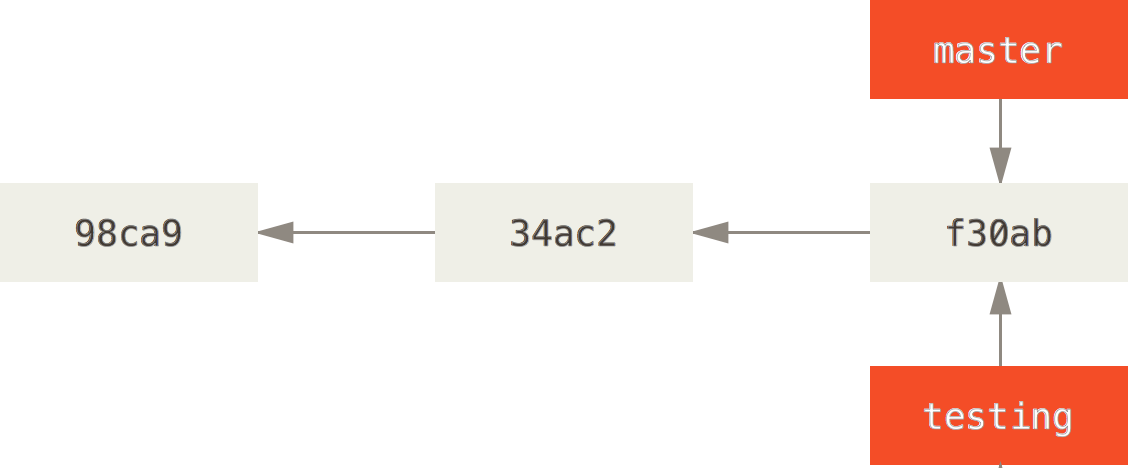
\includegraphics[width=\textwidth]{../fig/two-branches.png}
    \caption{Two branches pointing to the same commit.}
    \label{fig:1}
  \end{subfigure} 
  \hfill
  \begin{subfigure}[b]{0.4\textwidth}
    \centering
    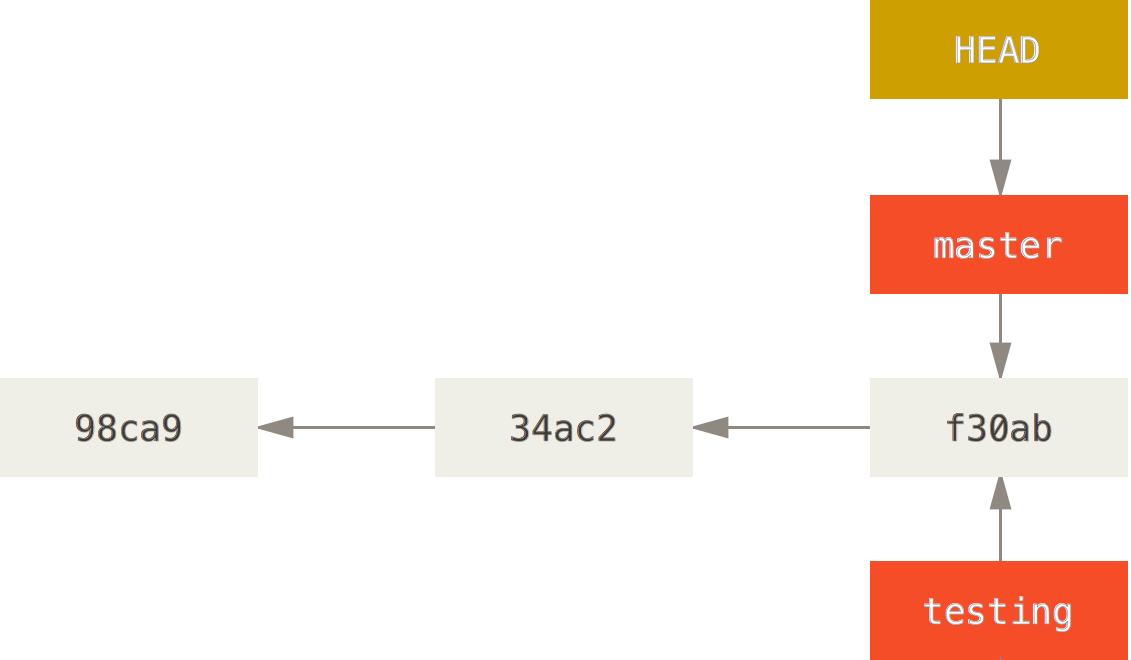
\includegraphics[width=\textwidth]{../fig/head-to-master.png}
    \caption{HEAD points to the current branch.}
    \label{fig:2}
  \end{subfigure}
\caption{Credit:  ProGit book, by Scott Chacon and Ben Straub, CC License.}
\end{figure}

To switch to the \texttt{testing} branch, you type:
%%begin.rcode git8.3, engine='bash', eval=FALSE
%$ git branch
%* master
%  testing
%$ git checkout testing
%Switched to branch 'testing'
%$ git branch
%  master
%* testing
%%end.rcode

Does it make sense that you switch branches by using \texttt{git checkout}?
What other situations would you use \texttt{git checkout}?  In particular,
can you use it to switch to commits that are unlabeled?  For example, if you
had the repository represented in Figure~\ref{fig:2}, how would the DAG change
if you typed:
%%begin.rcode git8.4, engine='bash', eval=FALSE
%$ git checkout 34ac2
%%end.rcode
How would you use \texttt{git checkout} to switch to the \texttt{testing}
branch?  What would happen to the DAG if you did that? 

If you had the above repository and issued the \texttt{git checkout 34ac2}
command, you would see something like this:
%%begin.rcode git8.5, engine='bash', eval=FALSE
%$ git checkout 34ac2
%Note: checking out '34ac2'.
%
%You are in 'detached HEAD' state. You can look around, make
%experimental changes and commit them, and you can discard any
%commits you make in this state without impacting any branches
%by performing another checkout.
%
%If you want to create a new branch to retain commits you create,
%you may do so (now or later) by using -b with the checkout
%command again. Example:
%
%  git checkout -b new_branch_name
%
%HEAD is now at 34ac2... 
%%end.rcode
Does this message make sense given what you've learned? What do you think
it means to be in a \textbf{detached HEAD} state?

\item Collaboration: using branches (work in pairs)

Work in pairs for the following. You should each be on your own computer,
but take turns watching each other type and talking through what you
are doing as you work through the questions together.

\begin{itemize}
\item \textbf{(Person A).} Create a new \textbf{feature} branch.\footnote{You can create and checkout a new branch in one step by typing \texttt{git checkout -b feature1}.}

%%begin.rcode git9, engine='bash', eval=FALSE
%$ git branch feature1
%$ git checkout feature1
%Switched to branch 'feature1'
%%end.rcode

Use \texttt{git status} to see what's going on. If everything looks
alright, it's time to implement your new feature.  For this feature, you
are going to print out the summary information, rather than the mean.

That is, change the line reading
%%begin.rcode git9.1, engine='bash', eval=FALSE
%mean(x)
%%end.rcode
so that it reads
%%begin.rcode git9.2, engine='bash', eval=FALSE
%summary(x)
%%end.rcode
Now add and commit your changes to your local repository.

Let's say that you have completed the implementation of your new feature
and that you've fully tested it.  Now you will want to merge your feature
branch back to your master branch.
%%begin.rcode git9.3, engine='bash', eval=FALSE
%$ git checkout master
%$ git merge feature1
%$ git branch -d feature1
%%end.rcode
Explain what each step does in terms of the underlying DAG.
Use \texttt{git branch --help} to see what the option
\texttt{-d} does.  How does this differ from what \texttt{-D} does?

Take a look at the DAG by typing:
%%begin.rcode git9.4, engine='bash', eval=FALSE
%$ git log --oneline --topo-order --graph
%%end.rcode

Finally, push your new changes to GitHub.

\item \textbf{(Person B).} Create a new \textbf{bugfix} branch.

First pull (i.e., fetch+merge) the work that Person A just pushed
to their GitHub repository. 

Use git status to see what’s going on. If everything looks alright,
it’s time to create a bugfix branch and fix the bug.

First create and checkout a new branch with one command:
%%begin.rcode git9.5, engine='bash', eval=FALSE
%$ git checkout -b bugfix1
%%end.rcode
Verify what happened with \texttt{status}.  Then replace \texttt{sin} with
\texttt{cos} in \texttt{stats.R}.  Save your changes, add the changed file
to the staging area, commit the changes to your repository.

Next merge your feature branch back to your master branch.
%%begin.rcode git9.6, engine='bash', eval=FALSE
%$ git checkout master
%$ git merge --no-ff bugfix1
%$ git branch -d bugfix1
%%end.rcode
Explain what each step does in terms of the underlying DAG.
Use \texttt{git merge --help} to see what the option \texttt{--no-ff}
does.  

Take a look at the DAG by typing:
%%begin.rcode git9.7, engine='bash', eval=FALSE
%$ git log --oneline --topo-order --graph
%%end.rcode
Can you see a loop that represents the work on the feature branch?
How does this differ from what happened when Person A merged their
feature branch?

If everything looks correct, push your new changes to GitHub.

\item \textbf{(Person A).} Make sure you can pull Person B's changes
from GitHub.  Take a look at the DAG by typing:
%%begin.rcode git9.8, engine='bash', eval=FALSE
%$ git log --oneline --topo-order --graph
%%end.rcode

\item \textbf{(Person A and Person B).} The feature and bugfix above
are obviously silly.  However, in practice, you will often work on
new features that take a long time to complete.  While you are working
on the feature, you may find that you decide that the feature is not
as desirable as you first thought.  If you work on the feature in
its own branch, you can discard that work easily without the code
polluting your main branch of development.

Similarly, bugfixes themselves may initially seem to require a significant
amount of new code.  However, after thinking about the bug longer, you may
realize that a much smaller change resolves the error.  If you were
working directly on your main branch, how would you simply remove all the
unnecessary code changes you made?

Can you think of other scenarios where isolating code changes to separate
lines of development would be desirable?

\end{itemize}


\item Collaboration: workflow (read and discuss in small groups)

At this point, you should have a basic understanding of how to create and
merge branches as well as how to work with collaborators using multiple
remotes.  Unlike many older version control systems, Git's model is
extremely flexible.  The inflexibility of older systems resulted in
everyone using the same workflows.  The added flexibility of Git makes it
possible to easily use many different types of workflows.  This means that
you will have to make a decision about which workflow you want to use for
every project you version control with Git.

If you are joining an existing project, you will often just adopt the
workflow that that project uses.  If you are starting a new project or
working on project where the workflow is being debated, you will need to
understand the benefits and disadvantages of the various workflows.

This is a complex issue.  Often experience will be required in order to
evaluate the merits of different workflows for different projects.
However, there are several basic workflow styles, which you should
understand.

Please read:

\begin{itemize}
\item \url{http://www.git-scm.com/book/en/v2/Git-Branching-Branching-Workflows}
\item \url{http://www.git-scm.com/book/en/v2/Distributed-Git-Distributed-Workflows}
\end{itemize}

Once you've finished reading the above links, please discuss. Do these workflows
make sense? Can you imagine/explain a scenario where one workflow might be
preferred over another?

For additional information about Git workflows, please see:
\begin{itemize}
\item \url{https://www.atlassian.com/git/tutorials/comparing-workflows}
\item \url{https://sandofsky.com/blog/git-workflow.html}
\item \url{https://matthew-brett.github.io/pydagogue/gitwash/development_workflow.html}
\end{itemize}

\end{enumerate}

\end{document}
